\begin{table}
	\caption{Mean average precision (mAP) and rank-n accuracy for person re-identification on synthesized images after performing shape/appearance swap. Input images from Deep Fashion test set. Note \cite{Esser:2018ue} is supervised w.r.t. shape.}
	\label{tab:reid}
	\begin{tabular}{l|cccr}
		\hline
		& mAP & rank-1 & rank-5 & rank-10 \\ \hline
		VU-Net \cite{Esser:2018ue} & 88.7\% & 87.5\% & {98.7}\% & {99.5}\% \\
		Ours & {90.3}\% & {89.4}\% &{98.2}\% & {99.2}\% \\ \hline
	\end{tabular}
\end{table}
\begin{table}
	\caption{Percentage of Correct Keypoints (PCK) for pose estimation on shape/appearance swapped generations.\;$\alpha$ is pixel distance divided by image diagonal. Note that \cite{Esser:2018ue} serves as upper bound, as it uses the groundtruth shape estimates.}
	%shape supervision.}
	\label{tab:pose}
	\begin{tabular}{l|cccr}
		\hline
		$\alpha$ & $2.5\%$ &  $5\%$ & $7.5\%$ & $10\%$ \\ \hline
		VU-Net \cite{Esser:2018ue} & {95.2}\% & {98.4}\% & {98.9}\% & {99.1}\% \\
		Ours & 85.6\% & 94.2\% &96.5\% & 97.4\% \\ \hline
	\end{tabular}
\end{table}
% BBC THUMB
%
\begin{figure}[t]
	\centering
	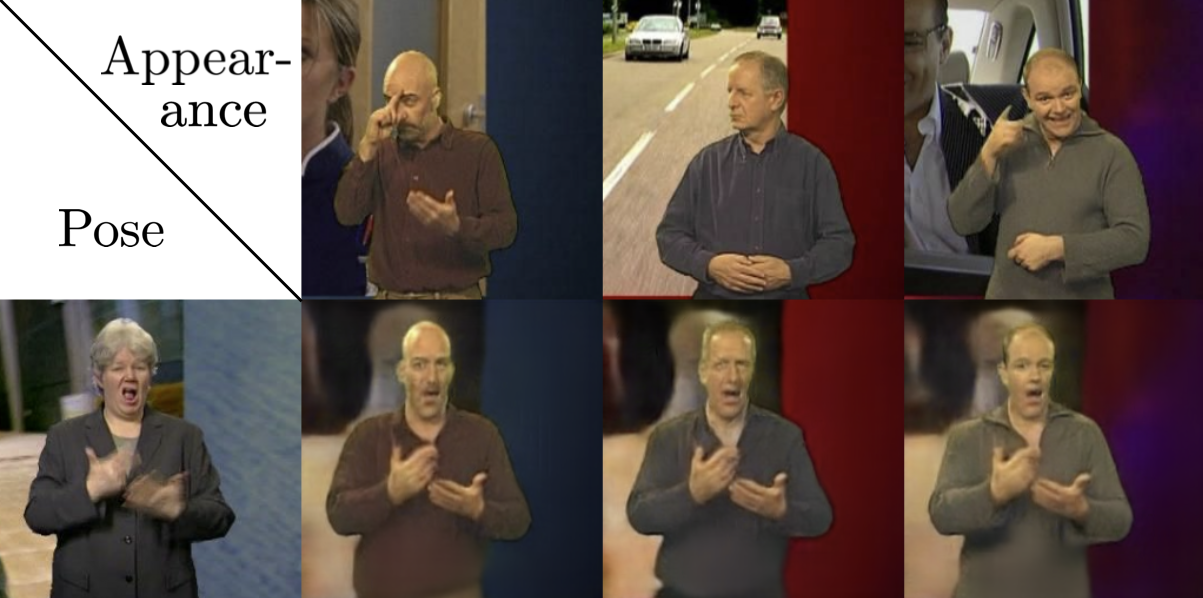
\includegraphics[trim={0cm 0cm 0cm 0cm},clip, width=1.\linewidth]{fig/bbcthumb}
	\caption{Video-to-video translation on BBC Pose. Top-row: target appearances, left: target pose.
	%The target appearances are from the train set, while the target pose is from the test set.
	Note that even fine details in shape are accurately captured. See supplementary for videos.}
	\label{fig:bbcthumb}
\end{figure}
